\documentclass[tikz]{standalone}

%\usepackage[export]{adjustbox}
%\usepackage{xcolor}
\usepackage{pst-barcode}
\usepackage{tikz}
\usetikzlibrary{positioning, arrows.meta, shapes, snakes, shadings}
%\usepackage{amsmath,amssymb,amsthm,pgfplots}

\definecolor{nuclei}{RGB}{169,201,237}
\definecolor{oil}{RGB}{132,132,130}

% Polychrome - Kelly
\definecolor{bead1}{RGB}{242,243,244}
\definecolor{bead2}{RGB}{175,35,55}
\definecolor{bead3}{RGB}{236,195,66}
\definecolor{bead4}{RGB}{41,103,160}
\definecolor{bead5}{RGB}{47,60,40}
\definecolor{bead6}{RGB}{150,180,55}
\definecolor{bead7}{RGB}{218,147,171}
\definecolor{bead8}{RGB}{229,137,50}
\definecolor{bead9}{RGB}{128,89,143}
\definecolor{bead10}{RGB}{126,51,31}
\definecolor{bead11}{RGB}{59,133,90}
\definecolor{bead12}{RGB}{192,178,134}

% Polychrome - Light24
\definecolor{light1}{RGB}{253,50,22}
\definecolor{light2}{RGB}{6,254,53}
\definecolor{light3}{RGB}{106,118,252}
\definecolor{light4}{RGB}{254,212,196}
\definecolor{light5}{RGB}{251,0,203}
\definecolor{light6}{RGB}{24,205,211}
\definecolor{light7}{RGB}{246,249,38}
\definecolor{light8}{RGB}{255,150,22}
\definecolor{light9}{RGB}{71,155,85}
\definecolor{light10}{RGB}{238,166,251}
\definecolor{light11}{RGB}{220,88,125}
\definecolor{light12}{RGB}{214,39,255}

\begin{document}

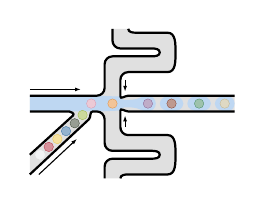
\begin{tikzpicture}
    %% whole channal
    \filldraw[draw=none, fill=oil!25]
        (0,1.05) --                  (0.85,1.05)
                 to[out=0, in=270]   (0.95,1.15)
                 --                  (0.95,1.45)
                 to[out=90, in=180]  (1.05,1.55)
                 --                  (1.55,1.55)
                 to[out=0, in=270]   (1.65,1.6)
                 to[out=90, in=0]    (1.55,1.65)
                 --                  (1.15,1.65)
                 to[out=180, in=270] (1.05,1.75)
                 --                  (1.05,1.9)
                 --                  (1.25,1.9)
                 to[out=270, in=180] (1.35,1.85)
                 --                  (1.75,1.85)
                 to[out=0, in=90]    (1.85,1.6)
                 to[out=270, in=0]   (1.75,1.35)
                 --                  (1.25,1.35)
                 to[out=180, in=90]  (1.15,1.25)
                 --                  (1.15,1.04)
                 to[out=270, in=180] (1.25,1.05)
                 --                  (2.6,1.05)
                 --                  (2.6,0.85)
                 --                  (1.25,0.85)
                 to[out=180, in=90]  (1.15,0.86)
                 --                  (1.15,0.65)
                 to[out=270, in=180] (1.25,0.55)
                 --                  (1.75,0.55)
                 to[out=0, in=90]    (1.85,0.3)
                 to[out=270, in=0]   (1.75,0.05)
                 --                  (1.25,0.05)
                 to[out=180, in=90]  (1.15,0)
                 --                  (0.95,0)
                 --                  (0.95,0.15)
                 to[out=90, in=180]  (1.05,0.25)
                 --                  (1.55,0.25)
                 to[out=0, in=270]   (1.65,0.3)
                 to[out=90, in=0]    (1.55,0.35)
                 --                  (1.05,0.35)
                 to[out=180, in=270] (0.95,0.45)
                 --                  (0.95,0.75)
                 to[out=90, in=0]    (0.85,0.85)
                 --                  (0.8,0.85)
                 to[out=180, in=45]  (0.75,0.75)
                 --                  (0,0.05)
                 --                  (0,0.3)
                 --                  (0.55,0.8)
                 to[out=45, in=0]    (0.5,0.85)
                 --                  (0,0.85)
                 --                  cycle;
    
    %% drop
    %%% curved drop
    \filldraw[draw=none, fill=nuclei!75]
        (0,1.05) --                  (0.85,1.05)
                 to[out=0, in=180]   (1.15,1.04)
                 to[out=270, in=180] (1.3,1)
                 to[out=0, in=180]   (1.5,1.05)
                 to[out=0, in=90]    (1.6,0.95)
                 to[out=270, in=0]   (1.5,0.85)
                 to[out=180, in=0]   (1.3,0.9)
                 to[out=180, in=90]  (1.15,0.86) 
                 to[out=180, in=0]   (0.85,0.85)
                 --                  (0,0.85)
                 --                  cycle;
    %%% following drops
    \filldraw[draw=none, fill=nuclei!75]
        (1.8,1.05) to[out=0, in=90]    (1.95,0.95)
                   to[out=270, in=0]   (1.8,0.85)
                   to[out=180, in=270]   (1.65,0.95)
                   to[out=90, in=180]  (1.8,1.05);
    \filldraw[draw=none, fill=nuclei!75]
        (2.15,1.05) to[out=0, in=90]    (2.3,0.95)
                   to[out=270, in=0]   (2.15,0.85)
                   to[out=180, in=270]   (2,0.95)
                   to[out=90, in=180]  (2.15,1.05);
    \filldraw[draw=none, fill=nuclei!75]
        (2.5,1.05) to[out=0, in=90]    (2.6,0.95)
                   to[out=270, in=0]   (2.5,0.85)
                   to[out=180, in=270]   (2.35,0.95)
                   to[out=90, in=180]  (2.5,1.05);
                 
    %% black outlines
    %%% bottom right
    \draw[thick]
        (1.15,0) to[out=90, in=180]  (1.25,0.05)
                 --                  (1.75,0.05)
                 to[out=0, in=270]   (1.85,0.3)
                 to[out=90, in=0]    (1.75,0.55)
                 --                  (1.25,0.55)
                 to[out=180, in=270] (1.15,0.65)
                 --                  (1.15,0.86)
                 to[out=90, in=180]  (1.25,0.85)
                 --                  (2.6,0.85);
    
    %%% bottom left
    \draw[thick]
        (0.95,0) --                  (0.95,0.15)
                 to[out=90, in=180]  (1.05,0.25)
                 --                  (1.55,0.25)
                 to[out=0, in=270]   (1.65,0.3)
                 to[out=90, in=0]    (1.55,0.35)
                 --                  (1.05,0.35)
                 to[out=180, in=270] (0.95,0.45)
                 --                  (0.95,0.75)
                 to[out=90, in=0]    (0.85,0.85)
                 --                  (0.8,0.85)
                 to[out=180, in=45]  (0.75,0.75)
                 --                  (0,0.05);
    \draw[thick]
        (0,0.3) --                   (0.55,0.8)
                to[out=45, in=0]     (0.5,0.85)
                --                   (0,0.85);
    
    %%% top right
    \draw[thick]
        (2.6,1.05) --                  (1.25,1.05)
                   to[out=180, in=270] (1.15,1.04)
                   --                  (1.15,1.25)
                   to[out=90, in=180]  (1.25,1.35)
                   --                  (1.75,1.35)
                   to[out=0, in=270]   (1.85,1.6)
                   to[out=90, in=0]    (1.75,1.85)
                   --                  (1.35,1.85)
                   to[out=180, in=270] (1.25,1.9);
    
    %%% top left
    \draw[thick]
        (0,1.05) --                  (0.85,1.05)
                 to[out=0, in=270]   (0.95,1.15)
                 --                  (0.95,1.45)
                 to[out=90, in=180]  (1.05,1.55)
                 --                  (1.55,1.55)
                 to[out=0, in=270]   (1.65,1.6)
                 to[out=90, in=0]    (1.55,1.65)
                 --                  (1.15,1.65)
                 to[out=180, in=270] (1.05,1.75)
                 --                  (1.05,1.9);
                 
    %% arrows
    \draw[->, -{Latex[length=0.75mm, width=0.5mm]}] (0, 1.13) -- (0.65, 1.13);
    \draw[->, -{Latex[length=0.75mm, width=0.5mm]}] (0.115, 0.05) -- (0.6, 0.5026);
    \draw[->, -{Latex[length=0.75mm, width=0.5mm]}] (1.21, 1.25) -- (1.21, 1.1);
    \draw[->, -{Latex[length=0.75mm, width=0.5mm]}] (1.21, 0.65) -- (1.21, 0.8);
                 
    % barcode beads
    \filldraw[ultra thin, draw=bead1, fill=bead1] (0.13, 0.3) circle (0.06);
    \node at (0.09,0.275) {\psbarcode[linecolor=black]{01234}{width=0.03 height=0.02}{ean5}};
    \filldraw[ultra thin, draw=bead2, fill=bead2!50] (0.24, 0.4) circle (0.06);
    \node at (0.2,0.375) {\psbarcode[linecolor=bead2]{14235}{width=0.03 height=0.02}{ean5}};
    \filldraw[ultra thin, draw=bead3, fill=bead3!50] (0.35, 0.5) circle (0.06);
    \node at (0.31,0.475) {\psbarcode[linecolor=bead3]{31254}{width=0.03 height=0.02}{ean5}};
    \filldraw[ultra thin, draw=bead4, fill=bead4!50] (0.46, 0.6) circle (0.06);
    \node at (0.42,0.575) {\psbarcode[linecolor=bead4]{54231}{width=0.03 height=0.02}{ean5}};
    \filldraw[ultra thin, draw=bead5, fill=bead5!50] (0.57, 0.7) circle (0.06);
    \node at (0.53,0.675) {\psbarcode[linecolor=bead5]{42315}{width=0.03 height=0.02}{ean5}};
    \filldraw[ultra thin, draw=bead6, fill=bead6!50] (0.67, 0.805) circle (0.06);
    \node at (0.63,0.78) {\psbarcode[linecolor=bead6]{76342}{width=0.03 height=0.02}{ean5}};
    \filldraw[ultra thin, draw=bead7, fill=bead7!50] (0.78, 0.95) circle (0.06);
    \node at (0.74,0.925) {\psbarcode[linecolor=bead7]{67531}{width=0.03 height=0.02}{ean5}};
    \filldraw[ultra thin, draw=bead8, fill=bead8!50] (1.05, 0.95) circle (0.06);
    \node at (1.01,0.925) {\psbarcode[linecolor=bead8]{23546}{width=0.03 height=0.02}{ean5}};
    \filldraw[ultra thin, draw=bead9, fill=bead9!50] (1.5, 0.95) circle (0.06);
    \node at (1.46,0.925) {\psbarcode[linecolor=bead9]{32485}{width=0.03 height=0.02}{ean5}};
    \filldraw[ultra thin, draw=bead10, fill=bead10!50] (1.8, 0.95) circle (0.06);
    \node at (1.76,0.925) {\psbarcode[linecolor=bead10]{76543}{width=0.03 height=0.02}{ean5}};
    \filldraw[ultra thin, draw=bead11, fill=bead11!50] (2.15, 0.95) circle (0.06);
    \node at (2.11,0.925) {\psbarcode[linecolor=bead11]{13572}{width=0.03 height=0.02}{ean5}};
    \filldraw[ultra thin, draw=bead12, fill=bead12!50] (2.475, 0.95) circle (0.06);
    \node at (2.435,0.925) {\psbarcode[linecolor=bead12]{23487}{width=0.03 height=0.02}{ean5}};
    
%    % barcode beads (3D like)
%    \shade[ultra thin, draw=bead1, ball color=light1!50] (0.13, 0.3) circle (0.06);
%    \node at (0.09,0.275) {\psbarcode[linecolor=black]{01234}{width=0.03 height=0.02}{ean5}};
%    \shade[ultra thin, draw=bead2, ball color=light2!50] (0.24, 0.4) circle (0.06);
%    \node at (0.2,0.375) {\psbarcode[linecolor=black]{14235}{width=0.03 height=0.02}{ean5}};
%    \shade[ultra thin, draw=bead3, ball color=light3!50] (0.35, 0.5) circle (0.06);
%    \node at (0.31,0.475) {\psbarcode[linecolor=black]{31254}{width=0.03 height=0.02}{ean5}};
%    \shade[ultra thin, draw=bead4, ball color=light4!50] (0.46, 0.6) circle (0.06);
%    \node at (0.42,0.575) {\psbarcode[linecolor=black]{54231}{width=0.03 height=0.02}{ean5}};
%    \shade[ultra thin, draw=bead5, ball color=light5] (0.57, 0.7) circle (0.06);
%    \node at (0.53,0.675) {\psbarcode[linecolor=black]{42315}{width=0.03 height=0.02}{ean5}};
%    \shade[ultra thin, draw=bead6, ball color=light6] (0.67, 0.805) circle (0.06);
%    \node at (0.63,0.78) {\psbarcode[linecolor=black]{76342}{width=0.03 height=0.02}{ean5}};
%    \shade[ultra thin, draw=bead7, ball color=light7] (0.78, 0.95) circle (0.06);
%    \node at (0.74,0.925) {\psbarcode[linecolor=black]{67531}{width=0.03 height=0.02}{ean5}};
%    \shade[ultra thin, draw=bead8, ball color=light8] (1.05, 0.95) circle (0.06);
%    \node at (1.01,0.925) {\psbarcode[linecolor=black]{23546}{width=0.03 height=0.02}{ean5}};
%    \shade[ultra thin, draw=bead9, ball color=light9] (1.5, 0.95) circle (0.06);
%    \node at (1.46,0.925) {\psbarcode[linecolor=black]{32485}{width=0.03 height=0.02}{ean5}};
%    \shade[ultra thin, draw=bead10, ball color=light10] (1.8, 0.95) circle (0.06);
%    \node at (1.76,0.925) {\psbarcode[linecolor=black]{76543}{width=0.03 height=0.02}{ean5}};
%    \shade[ultra thin, draw=bead11, ball color=light11] (2.15, 0.95) circle (0.06);
%    \node at (2.11,0.925) {\psbarcode[linecolor=black]{13572}{width=0.03 height=0.02}{ean5}};
%    \shade[ultra thin, draw=bead12, ball color=light12] (2.475, 0.95) circle (0.06);
%    \node at (2.435,0.925) {\psbarcode[linecolor=black]{23487}{width=0.03 height=0.02}{ean5}};
\end{tikzpicture}
    
\end{document}